%%% -*- coding: utf-8 -*-
\newpage

\chapter{Results}
\label{chap:results}


\begin{table}[]
\centering
\label{tab:cross-validation}
\caption{Weighted F2-Score (in percentage) for each model across 20-Fold Cross Validation).}
\begin{tabular}{l|l|l|l|l}
      & \multicolumn{1}{c|}{MLP} & \multicolumn{1}{c|}{LSTM} & \multicolumn{1}{c|}{SVM} & \multicolumn{1}{c}{KNN} \\ \hline
count & 20,0000                  & 20,0000                   & 20,0000                  & 20,0000                 \\ \hline
mean  & 99,0743                  & 98,9899                   & 98,8993                  & 96,4738                 \\ \hline
std   & 0,1349                   & 0,1174                    & 0,1347                   & 0,2915                  \\ \hline
min   & 98,7945                  & 98,7943                   & 98,5445                  & 95,6932                 \\ \hline
25\%  & 99,0073                  & 98,9175                   & 98,8499                  & 96,3585                 \\ \hline
50\%  & 99,0962                  & 98,9848                   & 98,9174                  & 96,4108                 \\ \hline
75\%  & 99,1708                  & 99,0684                   & 98,9756                  & 96,6564                 \\ \hline
max   & 99,2885                  & 99,1915                   & 99,0836                  & 96,9448                
\end{tabular}
\end{table}

\begin{table}[]
\centering
\label{tab:test-2k}
\caption{Test on the NPDI 2k-pornography dataset results, shown in absolute values).}
\begin{tabular}{l|l|l|l|l|l}
             & precision & recall & f1-score & f2-score & support    \\ \hline
Safe         & 0,9665    & 0,8080 & 0,8802   & 0,9411   & 1.000,0000 \\ \hline
Sensitive    & 0,8351    & 0,9720 & 0,8983   & 0,8354   & 1.000,0000 \\ \hline
weighted avg & 0,9008    & 0,8900 & 0,8893   & 0,8883   & 2.000,0000
\end{tabular}
\end{table}

\begin{table}[]
\centering
\label{tab:test-general}
\caption{Test subset results, shown in absolute values).}
\begin{tabular}{l|l|l|l|l|l}
             & precision & recall & f1-score & f2-score & support                         \\ \hline
Safe         & 0,9895    & 0,9906 & 0,9900   & 0,9897   & 5973,0000                       \\ \hline
Sensitive    & 0,9906    & 0,9895 & 0,9900   & 0,9904   & 5973,0000                       \\ \hline
weighted avg & 0,9900    & 0,9900 & 0,9900   & 0,9900   & \multicolumn{1}{l}{11946,0000}
\end{tabular}
\end{table}

\begin{table}[]
\centering
\label{tab:test-porn}
\caption{Results testing pornography only, shown in absolute values).}
\begin{tabular}{l|l|l|l|l|l}
             & precision & recall & f1-score & f2-score & support    \\ \hline
Safe         & 0,9947    & 0,9902 & 0,9925   & 0,9939   & 5737,0000  \\ \hline
Sensitive    & 0,9903    & 0,9948 & 0,9925   & 0,9911   & 5737,0000  \\ \hline
weighted avg & 0,9925    & 0,9925 & 0,9925   & 0,9925   & 11474,0000
\end{tabular}
\end{table}

\begin{table}[]
\centering
\label{tab:test-gore}
\caption{Results testing gore videos only, shown in absolute values).}
\begin{tabular}{l|l|l|l|l|l}
             & precision & recall & f1-score & f2-score & support  \\ \hline
Safe         & 0,8764    & 0,9915 & 0,9304   & 0,8834   & 236,0000 \\ \hline
Sensitive    & 0,9902    & 0,8602 & 0,9206   & 0,9661   & 236,0000 \\ \hline
weighted avg & 0,9333    & 0,9258 & 0,9255   & 0,9248   & 472,0000
\end{tabular}
\end{table}


\begin{figure*}[!ht]
    \centering
    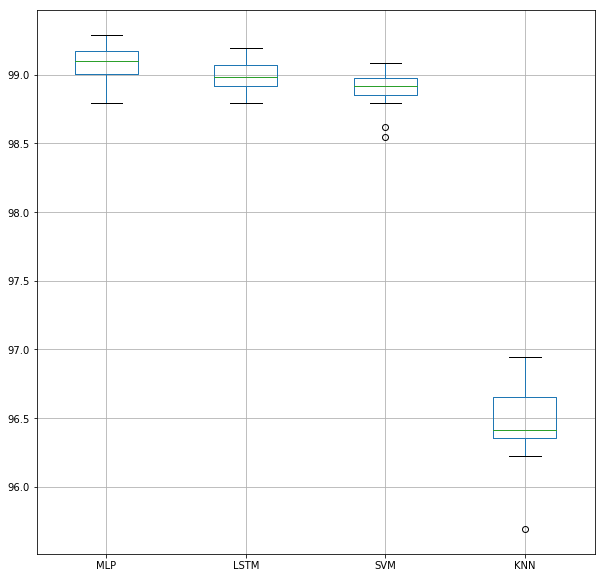
\includegraphics[width=0.9\textwidth]{img/results/boxplot.png}
    \caption{Boxplot of the results of each model throughout the 20-fold cross validation.}
    \label{fig:results-boxplot}
\end{figure*}

\begin{figure*}[!ht]
    \centering
    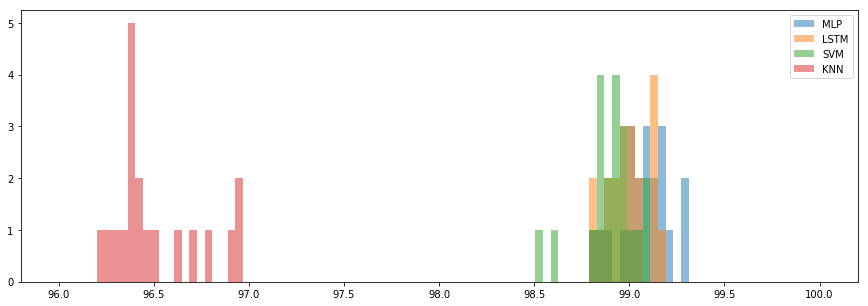
\includegraphics[width=0.9\textwidth]{img/results/histogram.png}
    \caption{Histogram of the results of each model throughout the 20-fold cross validation.}
    \label{fig:results-histogram}
\end{figure*}

\begin{figure*}[!ht]
    \centering
    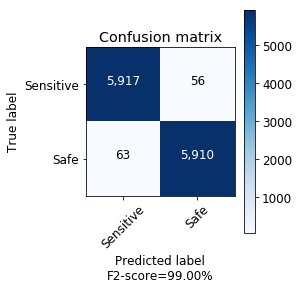
\includegraphics[width=0.49\textwidth]{img/results/MLP-TEST.png}
    \caption{Confusion matrix of the predictions of the best model in the test subset.}
    \label{fig:cf-test}
\end{figure*}

\begin{figure*}[!ht]
    \centering
    \begin{subfigure}[b]{0.49\textwidth}
        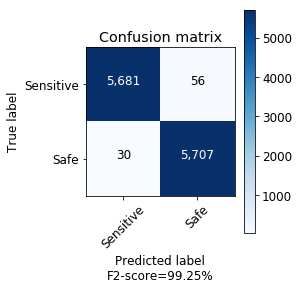
\includegraphics[width=0.93\textwidth]{img/results/MLP-TEST-PORN.png}
        \caption{Confusion matrix of the model on the pornography videos of the test subset.}
        \label{fig:cf-test-porn}
    \end{subfigure}
    \begin{subfigure}[b]{0.49\textwidth}
        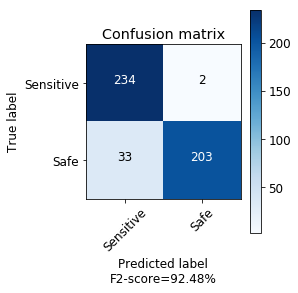
\includegraphics[width=0.90\textwidth]{img/results/MLP-TEST-GORE.png}
        \caption{Confusion matrix of the model on the gore videos of the test subset.}
        \label{fig:cf-test-gore}
    \end{subfigure}
\end{figure*}

\begin{figure*}[!ht]
    \centering
    \begin{subfigure}[b]{0.49\textwidth}
        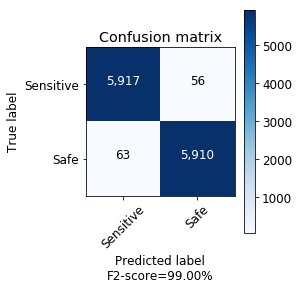
\includegraphics[width=0.94\textwidth]{img/results/MLP-TEST-IMAGE-ONLY.png}
        \caption{Confusion matrix of the model on the test subset using only image features.}
        \label{fig:cf-test-image}
    \end{subfigure}
    \begin{subfigure}[b]{0.49\textwidth}
        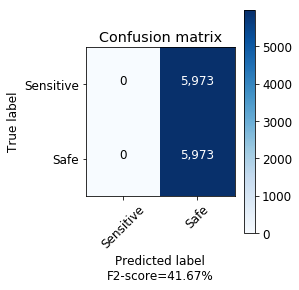
\includegraphics[width=0.94\textwidth]{img/results/MLP-TEST-AUDIO-ONLY.png}
        \caption{Confusion matrix of the model on the test subset using only audio features.}
        \label{fig:cf-test-audio}
    \end{subfigure}
\end{figure*}

\begin{figure*}[!ht]
    \centering
    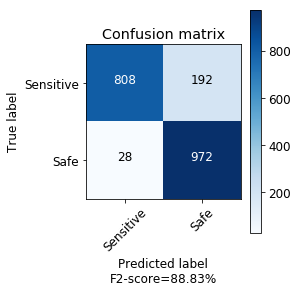
\includegraphics[width=0.49\textwidth]{img/results/MLP-2K-TEST.png}
    \caption{Confusion matrix of the predictions of the best model in the NPDI 2k-pornography dataset.}
    \label{fig:cf-test-2k}
\end{figure*}


\begin{figure*}[!ht]
    \centering
    \begin{subfigure}[b]{0.49\textwidth}
        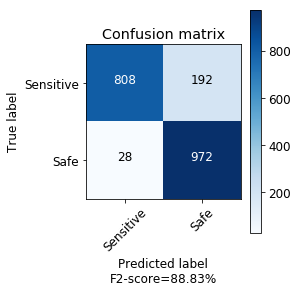
\includegraphics[width=0.94\textwidth]{img/results/MLP-2K-TEST-IMAGE-ONLY.png}
        \caption{Confusion matrix of the model on the NPDI 2k-pornography dataset using only image features.}
        \label{fig:cf-test-2k-image}
    \end{subfigure}
    \begin{subfigure}[b]{0.49\textwidth}
        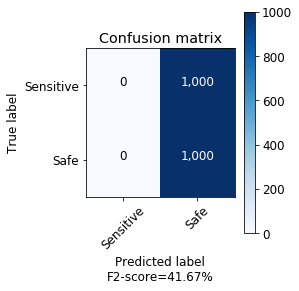
\includegraphics[width=0.94\textwidth]{img/results/MLP-2K-TEST-AUDIO-ONLY.png}
        \caption{Confusion matrix of the model on the NPDI 2k-pornography dataset using only audio features.}
        \label{fig:cf-test-2k-audio}
    \end{subfigure}
\end{figure*}

\section{Discussion}\label{sec:discussion}
% Discutir vantagens e desvantagens do eraly fusion por causa de forçar o modelo a aprender uma mdeia de cada e depois combinar
% Possibilidades pra so ter aprendido imagens:
%Diferença no tamanho das deatures de audio e frames
%Diferença pra early e late fusion
%Só a mlp aprendeu isso
%Features ruins de audio
% Receptive field pra áudio pequeno
% Audio n faz diferença ***: perguntar pra paulo oq ele quis dizer
\section{Analysis cases}\label{sec:experiments-discussion}